\documentclass{article}
\usepackage[utf8]{inputenc}
\usepackage{tikz}
\usetikzlibrary{fit,arrows.meta,external,math,decorations.pathmorphing}
\usepackage{amsmath,amsfonts,amssymb}
\usepackage{xcolor}
\usetikzlibrary{matrix}
\usepackage{xcolor}
\usepackage{subcaption}


\title{CSuite Graphs}
\author{Adam Foster}
\date{Septeber 2022}

\begin{document}

\maketitle

\begin{figure}
\begin{subfigure}{0.5\columnwidth}
    \centering
    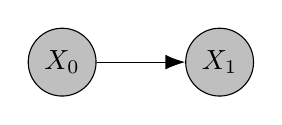
\begin{tikzpicture}
	\node (y) [draw, circle, fill=lightgray] at (-1, 1) {$X_0$};
	\node (z) [draw, circle,fill=lightgray] at (1, 1) {$X_1$};
	\draw[-{Latex[length=2.5mm]}] (y) -> (z);
	\end{tikzpicture}
    \caption{Two node}\label{fig:two_node_pgm}
\end{subfigure}
\begin{subfigure}{0.5\columnwidth}
    \centering
    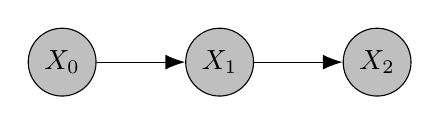
\begin{tikzpicture}
	\node (y) [draw, circle, fill=lightgray] at (-1, 1) {$X_0$};
	\node (z) [draw, circle,fill=lightgray] at (1, 1) {$X_1$};
	\node (a) [draw, circle,fill=lightgray] at (3, 1) {$X_2$};
	\draw[-{Latex[length=2.5mm]}] (y) -> (z);
	\draw[-{Latex[length=2.5mm]}] (z) -> (a);
	\end{tikzpicture}
    \caption{Chain}\label{fig:chain_pgm}
\end{subfigure}
\begin{subfigure}{0.5\columnwidth}
    \centering
    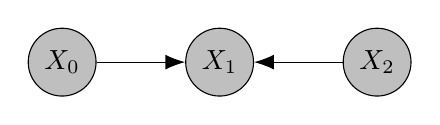
\begin{tikzpicture}
	\node (y) [draw, circle, fill=lightgray] at (-1, 1) {$X_0$};
	\node (z) [draw, circle,fill=lightgray] at (1, 1) {$X_1$};
	\node (a) [draw, circle,fill=lightgray] at (3, 1) {$X_2$};
	\draw[-{Latex[length=2.5mm]}] (y) -> (z);
	\draw[-{Latex[length=2.5mm]}] (a) -> (z);
	\end{tikzpicture}
    \caption{Collider}\label{fig:collider_pgm}
\end{subfigure}
\begin{subfigure}{0.5\columnwidth}
    \centering
    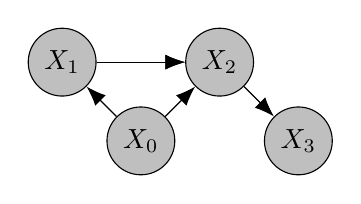
\begin{tikzpicture}
	\node (y) [draw, circle, fill=lightgray] at (-1, 1) {$X_1$};
	\node (z) [draw, circle,fill=lightgray] at (1, 1) {$X_2$};
	\draw[-{Latex[length=2.5mm]}] (y) -> (z);
	\node (a) [draw, circle, fill=lightgray] at (0, 0) {$X_0$};
	\node (b) [draw, circle,fill=lightgray] at (2, 0) {$X_3$};
	\draw[-{Latex[length=2.5mm]}] (y) -> (z);
	\draw[-{Latex[length=2.5mm]}] (a) -> (z);
	\draw[-{Latex[length=2.5mm]}] (a) -> (y);
	\draw[-{Latex[length=2.5mm]}] (z) -> (b);
	\end{tikzpicture}
    \caption{Nonlin. Simpson}\label{fig:nonlin_simpson_pgm}
\end{subfigure}
\begin{subfigure}{0.5\columnwidth}
    \centering
    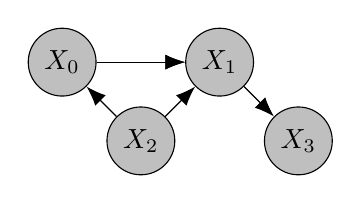
\begin{tikzpicture}
	\node (y) [draw, circle, fill=lightgray] at (-1, 1) {$X_0$};
	\node (z) [draw, circle,fill=lightgray] at (1, 1) {$X_1$};
	\draw[-{Latex[length=2.5mm]}] (y) -> (z);
	\node (a) [draw, circle, fill=lightgray] at (0, 0) {$X_2$};
	\node (b) [draw, circle,fill=lightgray] at (2, 0) {$X_3$};
	\draw[-{Latex[length=2.5mm]}] (y) -> (z);
	\draw[-{Latex[length=2.5mm]}] (a) -> (z);
	\draw[-{Latex[length=2.5mm]}] (a) -> (y);
	\draw[-{Latex[length=2.5mm]}] (z) -> (b);
	\end{tikzpicture}
    \caption{Nonlin. Simpson (2)}\label{fig:nonlin_simpson_pgm}
\end{subfigure}
\begin{subfigure}{0.5\columnwidth}
    \centering
    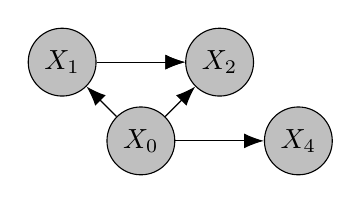
\begin{tikzpicture}
	\node (y) [draw, circle, fill=lightgray] at (-1, 1) {$X_1$};
	\node (z) [draw, circle,fill=lightgray] at (1, 1) {$X_2$};
	\draw[-{Latex[length=2.5mm]}] (y) -> (z);
	\node (a) [draw, circle, fill=lightgray] at (0, 0) {$X_0$};
	\node (b) [draw, circle,fill=lightgray] at (2, 0) {$X_4$};
	\draw[-{Latex[length=2.5mm]}] (y) -> (z);
	\draw[-{Latex[length=2.5mm]}] (a) -> (z);
	\draw[-{Latex[length=2.5mm]}] (a) -> (y);
	\draw[-{Latex[length=2.5mm]}] (a) -> (b);
	\end{tikzpicture}
    \caption{Symprod. Simpson}\label{fig:symprod_simpson_pgm}
\end{subfigure}
\vspace{15pt}
\begin{subfigure}{0.5\columnwidth}
    \centering
    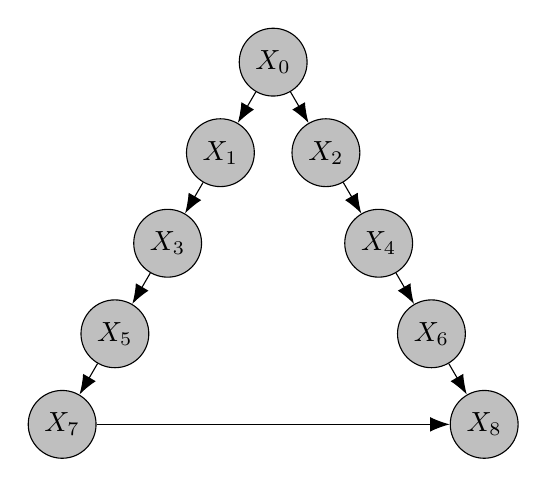
\begin{tikzpicture}
	\node (x1) [draw, circle, fill=lightgray] at (0,0) {$X_0$};
	\node (x2) [draw, circle, fill=lightgray] at (-.67, -1.15) {$X_1$};
	\node (x3) [draw, circle, fill=lightgray] at (.67, -1.15) {$X_2$};
	\node (x4) [draw, circle, fill=lightgray] at (-1.34, -2.3) {$X_3$};
	\node (x5) [draw, circle, fill=lightgray] at (1.34, -2.3) {$X_4$};
	\node (x6) [draw, circle, fill=lightgray] at (-2.01, -3.45) {$X_5$};
	\node (x7) [draw, circle, fill=lightgray] at (2.01, -3.45) {$X_6$};
	\node (x8) [draw, circle, fill=lightgray] at (-2.68, -4.6) {$X_7$};
	\node (x9) [draw, circle, fill=lightgray] at (2.68, -4.6) {$X_8$};
	\draw[-{Latex[length=2.5mm]}] (x1) -> (x2);
	\draw[-{Latex[length=2.5mm]}] (x1) -> (x3);
	\draw[-{Latex[length=2.5mm]}] (x2) -> (x4);
	\draw[-{Latex[length=2.5mm]}] (x3) -> (x5);
	\draw[-{Latex[length=2.5mm]}] (x4) -> (x6);
	\draw[-{Latex[length=2.5mm]}] (x5) -> (x7);
	\draw[-{Latex[length=2.5mm]}] (x6) -> (x8);
	\draw[-{Latex[length=2.5mm]}] (x7) -> (x9);
	\draw[-{Latex[length=2.5mm]}] (x8) -> (x9);
	\end{tikzpicture}
    \caption{Large backdoor.}\label{fig:large_backdoor_pgm}
\end{subfigure}
\begin{subfigure}{0.5\columnwidth}
    \centering
    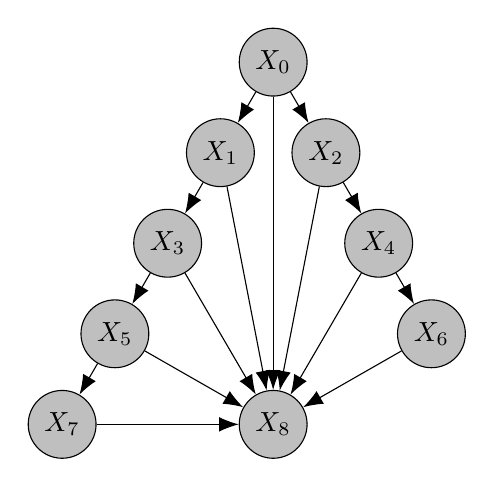
\begin{tikzpicture}
	\node (x1) [draw, circle, fill=lightgray] at (0,0) {$X_0$};
	\node (x2) [draw, circle, fill=lightgray] at (-.67, -1.15) {$X_1$};
	\node (x3) [draw, circle, fill=lightgray] at (.67, -1.15) {$X_2$};
	\node (x4) [draw, circle, fill=lightgray] at (-1.34, -2.3) {$X_3$};
	\node (x5) [draw, circle, fill=lightgray] at (1.34, -2.3) {$X_4$};
	\node (x6) [draw, circle, fill=lightgray] at (-2.01, -3.45) {$X_5$};
	\node (x7) [draw, circle, fill=lightgray] at (2.01, -3.45) {$X_6$};
	\node (x8) [draw, circle, fill=lightgray] at (-2.68, -4.6) {$X_7$};
	\node (x9) [draw, circle, fill=lightgray] at (0, -4.6) {$X_8$};
	\draw[-{Latex[length=2.5mm]}] (x1) -> (x2);
	\draw[-{Latex[length=2.5mm]}] (x1) -> (x3);
	\draw[-{Latex[length=2.5mm]}] (x2) -> (x4);
	\draw[-{Latex[length=2.5mm]}] (x3) -> (x5);
	\draw[-{Latex[length=2.5mm]}] (x4) -> (x6);
	\draw[-{Latex[length=2.5mm]}] (x5) -> (x7);
	\draw[-{Latex[length=2.5mm]}] (x6) -> (x8);
	\draw[-{Latex[length=2.5mm]}] (x7) -> (x9);
	\draw[-{Latex[length=2.5mm]}] (x8) -> (x9);
	\draw[-{Latex[length=2.5mm]}] (x1) -> (x9);
	\draw[-{Latex[length=2.5mm]}] (x2) -> (x9);
	\draw[-{Latex[length=2.5mm]}] (x3) -> (x9);
	\draw[-{Latex[length=2.5mm]}] (x4) -> (x9);
	\draw[-{Latex[length=2.5mm]}] (x5) -> (x9);
	\draw[-{Latex[length=2.5mm]}] (x6) -> (x9);
	\end{tikzpicture}
    \caption{Weak arrows. }\label{fig:weak_arrows_pgm}
\end{subfigure}
\vspace{15pt}
\begin{subfigure}{\columnwidth}
    \centering
    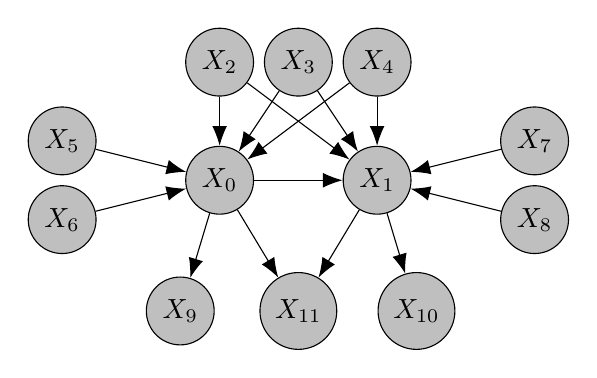
\begin{tikzpicture}
	\node (x1) [draw, circle, fill=lightgray] at (-1, 1) {$X_0$};
	\node (x2) [draw, circle,fill=lightgray] at (1, 1) {$X_1$};
	\node (x3) [draw, circle,fill=lightgray] at (-1, 2.5) {$X_2$};
	\node (x4) [draw, circle,fill=lightgray] at (0, 2.5) {$X_3$};
	\node (x5) [draw, circle,fill=lightgray] at (1, 2.5) {$X_4$};
	\node (x6) [draw, circle,fill=lightgray] at (-3, 1.5) {$X_5$};
	\node (x7) [draw, circle,fill=lightgray] at (-3, .5) {$X_6$};
	\node (x8) [draw, circle,fill=lightgray] at (3, 1.5) {$X_7$};
	\node (x9) [draw, circle,fill=lightgray] at (3, .5) {$X_8$};
	\node (x10) [draw, circle,fill=lightgray] at (-1.5, -.66) {$X_{9}$};
	\node (x12) [draw, circle,fill=lightgray] at (0, -.66) {$X_{11}$};
	\node (x11) [draw, circle,fill=lightgray] at (1.5, -.66) {$X_{10}$};
	\draw[-{Latex[length=2.5mm]}] (x1) -> (x2);
	\draw[-{Latex[length=2.5mm]}] (x3) -> (x1);
	\draw[-{Latex[length=2.5mm]}] (x3) -> (x2);
	\draw[-{Latex[length=2.5mm]}] (x4) -> (x1);
	\draw[-{Latex[length=2.5mm]}] (x4) -> (x2);
	\draw[-{Latex[length=2.5mm]}] (x5) -> (x1);
	\draw[-{Latex[length=2.5mm]}] (x5) -> (x2);
	\draw[-{Latex[length=2.5mm]}] (x6) -> (x1);
	\draw[-{Latex[length=2.5mm]}] (x7) -> (x1);
	\draw[-{Latex[length=2.5mm]}] (x8) -> (x2);
	\draw[-{Latex[length=2.5mm]}] (x9) -> (x2);
	\draw[-{Latex[length=2.5mm]}] (x1) -> (x10);
	\draw[-{Latex[length=2.5mm]}] (x2) -> (x11);
	\draw[-{Latex[length=2.5mm]}] (x1) -> (x12);
	\draw[-{Latex[length=2.5mm]}] (x2) -> (x12);
	\end{tikzpicture}
    \caption{Mixed confounding}\label{fig:mixed_confounding_pgm}
\end{subfigure}
    \caption{CSuite graphs.}
    \label{fig:csuite_pgms}
\end{figure}


\end{document}
